
\chapter{绪论}
\label{Chapter_introduction} % 不建议用数字序号设置标签

\section{引言}

机器翻译(machine translation,MT)是建立在语言学、数学和计算机技术这三门学科的基础之上,用计算机将一种自然语言(源语言,source language)自动翻译成另一种自然语言(目标语言,target language)的一门学科和技术[\cite{zhangzong:2013,zong:2013}]。

机器翻译兴起于20世纪50年代初。1946年世界上第一台计算机ENIAC诞生以后,英国工程师A. D. Booth和美国洛克菲勒基金会副总裁W. Weaver提出了利用计算机进行自动翻译的设想。1949年W. Weaver发表了以 ``Translation'' 为题目的备忘录,正式提出了机器翻译问题。从这时起,我们对机器翻译的研究和探索就从来没有终止过。
在过去的六十多年中,机器翻译研究经历了认识、深入、停滞到再发展的曲折历程[\cite{Hutchins:2007}],同时也促进了人们对语言、知识和智能的深入理解和思考。在机器翻译研究的历史上,我们大致可以将机器翻译方法分为如下四类:直接转换法、基于规则的转换翻译方法、基于中间语言的翻译方法、基于语料库的翻译方法。其中,基于语料库的翻译方法又可以分为基于记忆的翻译方法、基于实例的翻译方法、统计翻译方法和神经网络翻译方法。近年来,基于统计的翻译方法和神经网络翻译方法逐渐成为机器翻译的主流方法。

统计机器翻译的开山之作是IBM的P. F. Brown等人在Computational Linguistics上发表的“统计机器翻译方法”[\cite{Brown:1990}]和1993年发表的“统计机器翻译的数学:参数估计”[\cite{Brown:1993}]两篇论文。在这两篇论文中他们提出并论证了基于统计方法的机器翻译模型。从此,伴随着计算机硬件技术的快速发展和网络技术的迅速普及和应用,机器翻译进入了空前辉煌的发展时期。

经过二十多年的发展,统计机器翻译取得了一系列丰硕的成果,基于词的方法[\cite{Brown:1990,Brown:1993}]、基于短语的方法[\cite{Marcu:2002,Koehn:2003}]以及基于句法的方法[\cite{Galley:2004,Chiang:2005,Galley:2006,LiuYang:2006}]相继被提出,翻译过程中使用到的信息也在向深度和广度两个方向拓展[\cite{Zhai:2012,TuMei:2013,TuMei:2014}]。然而,由于统计机器翻译方法采用离散符号来表示翻译知识,导致它还存在一些难以回避的问题,如长句和复杂句式的处理问题,弱规范甚至非规范化文本的翻译问题,一些专业领域双语资源缺乏问题,根据用户反馈在线学习问题,机器翻译评测指标问题,如何有效应用统计机器翻译的问题等。

与此同时,神经网络的方法在沉寂多年后逐渐开始复兴,并在语音和图像等领域大获成功。于是研究人员开始尝试使用神经网络中的连续向量表示来对翻译过程进行建模。经过短短两三年的发展,该方法就达到了与传统统计机器翻译方法相媲美的效果[\cite{Kalchbrenner:2013,Sutskever:2014,Cho:2014,Bahdanau:2015}]。当然,新的神经网络机器翻译也面临着很多新的问题和挑战,需要人们进行更加深入的研究,如重复翻译与漏翻译,词对齐效果不理想,流畅性好而忠实度差的问题等。

在工业界,各大互联网和软件公司,如谷歌、微软、百度、搜狗等,也都相继推出了以统计机器翻译或神经网络机器翻译为核心的在线翻译服务。这充分说明统计机器翻译和神经网络机器翻译已经成为当今机器翻译领域的核心主流技术。随着国际社会全球化进程的不断加快和国际交流的日益频繁,人们对不同语言之间的翻译需求越来越迫切,机器翻译研究也愈加具有应用价值。

\section{论文的研究背景和意义}

计算机辅助翻译(computer-assisted translation,CAT)可以帮助专业译员优质、高效、轻松地完成翻译工作。已有的计算机辅助翻译方法往往不依赖于机器翻译,而是在人的参与下完成整个翻译过程。基于翻译记忆(translation memory,TM)的计算机辅助翻译软件仍具有得天独厚的优势。这是因为在特定领域中,如果待翻译文本与记忆库中的文本匹配程度很高时,翻译记忆的译文质量明显优于机器翻译的译文。随着机器翻译技术的不断发展,虽然通过引入机器翻译来辅助专业译员以提高人工翻译效率是行业的必然趋势,但在很多时候,专业译员往往不想花费太多时间阅读自动译文。在这种情况下,机器翻译的作用极其有限。

与一般用于概要阅读的机器翻译系统相比,包含以谷歌为例的在线翻译系统和其它形式的私有定制翻译系统,作为一种生产力工具,译员对面向辅助翻译的机器翻译系统有更多的期待和要求。目前这方面的研究还处于萌芽阶段,还没有出现专门面向计算机辅助翻译的统计机器翻译系统。在机器翻译领域,较早被提出和实现的人机交互式机器翻译方法主要是译后编辑(post-editing,PE)和交互式机器翻译(interactive machine translation,IMT)。

译后编辑指通过人工直接修改机器翻译的自动译文来完成翻译,是最简单的人机交互方式。计算机辅助翻译工具如Trados等通常支持谷歌翻译等API来直接获取机器翻译的自动译文,因此译后编辑也是目前最流行的辅助形式。如果机器翻译的自动译文质量较高,人工修改量就比较少,这种方式可以有效提升译员的生产效率。但如果自动译文质量较差,修改的代价可能高于直接翻译,则这种方式并不能提高人工翻译效率。

交互式机器翻译指系统根据用户已翻译的部分译文,动态生成后续译文供用户参考,译员仅在翻译过程中选择可接受的部分即可。与译后编辑相比,交互式机器翻译系统对技术实现有更高的要求,如从左至右的强制解码。同时,译员也被要求从左至右进行翻译,这显然给用户带来了明显的额外负担,也与人工翻译习惯不相符合。因此,目前流行的在线翻译系统和计算机辅助翻译工具并不支持交互式机器翻译模式。

为了达到让机器翻译来辅助人工翻译以提高生产效率的目的,结合实际的人工翻译过程和现有机器翻译技术水平,我们认为目前现有的译后编辑和交互式机器翻译技术是远远不够的。

基于这一研究背景,本文致力于研究和改善专门面向计算机辅助翻译的机器翻译,在后文中我们称之为人机交互式机器翻译(human-computer interactive machine translation, HCIMT)。有别于现有的以概要阅读为主要目标的机器翻译,人机交互式机器翻译的优化目标是在人工翻译场景中提高生产效率,同时提供良好的人机交互体验。因此,本文的主要内容是围绕提高专业译员的生产效率,为人机交互式机器翻译有针对性地提出解决方法。

在详细、深入分析现有方法的优缺点基础之上,本论文尝试回答三个问题:

\begin{itemize}
	\item 目前的机器翻译自动译文质量尚未达到人工翻译场景的用户期望,而已有的译后编辑和交互式机器翻译的人机交互方式过度依赖自动译文质量。如何让专业译员更有效地利用现有机器翻译来提升翻译效率?
	
	\item 术语广泛存在于具体的领域语料中,专业译员在术语翻译上所用的时间多达75\% [\cite{Austermuhl:2014}]。可见术语翻译对于人机交互式机器翻译至关重要。如何改善对于专业领域至关重要的术语翻译质量?
	
	\item 复纠正相同错误的乏味感让使用机器翻译的专业译员感到沮丧。如何有效利用译员反馈的翻译结果实时改善机器翻译的译文质量?
	
	\item 为此,本文开展了如下三项研究工作:(1)研究融合统计机器翻译知识的中文输入方法;(2)提出融合术语识别边界信息的术语翻译方法;(3)探索基于随机森林的统计翻译模型在线学习方法。最后,我们设计和实现了融合机器翻译和计算机辅助翻译的人机交互式机器翻译系统,并总结了开发过程中遇到的关键问题和应对策略。
\end{itemize}

\section{论文的组织}

\begin{figure}[!htbp]
	\centering
	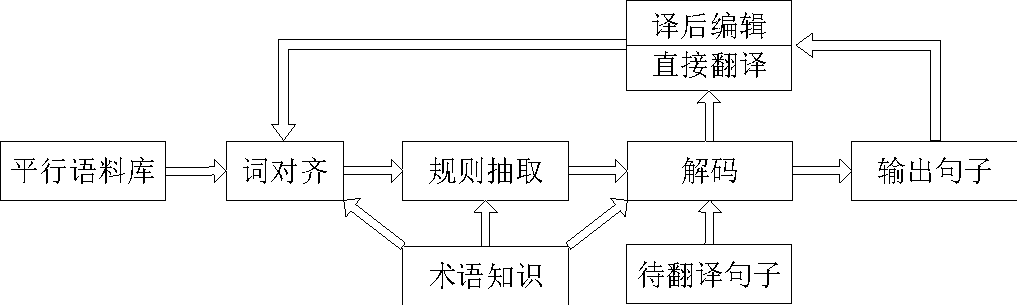
\includegraphics[width=0.95\textwidth]{Figure/Figure_1_1.pdf}
	\caption{人机交互式机器翻译流程简图}
	\label{Fig_imt_procedure}
\end{figure}

人机交互式机器翻译流程如图\ref{Fig_imt_procedure}所示,本文其余各章的组织如下:

第2章为机器翻译技术和人机交互式机器翻译方法综述。在这一章中先给出统计机器翻译和神经网络机器翻译的问题定义,并简要介绍机器翻译发展至今所出现的主要模型。再详细介绍人机交互式机器翻译方法。还将详细分析目前机器翻译和人机交互式机器翻译方法在人工翻译场景中存在的问题,并引出本论文所要开展的工作。该章是整篇论文的基础。

第3章提出了一种融合统计机器翻译技术的中文输入方法。为了充分发挥机器翻译知识在人工翻译场景中的作用,同时改善机器翻译人机交互体验,在该章中,我们提出的面向计算机辅助翻译的中文输入方法将统计翻译中的翻译规则、翻译假设列表和翻译结果候选列表等相关信息融合进输入法的对数线性模型,利用较少的按键就能生成准确的译文结果。另外,该输入方法的N元文法提示模型根据翻译结果候选列表生成译文提示,使译员更方便地选择统计翻译的高质量片断。此外,为了指导统计机器翻译系统生成更适合输入方法的翻译结果,我们提出了面向输入方法的译文自动评价指标,用于统计机器翻译系统的最小错误率训练。人工翻译实验结果表明,该输入法大幅减少大幅减少翻译人员的译文修改强度,显著提高翻译效率和译文质量。提出的自动评价指标能使该输入方法利用更合适的统计翻译结果,进一步提升人工翻译效率。提出的输入法作用于图1.1中的“译后编辑/直接翻译”环节,而面向输入方法的译文自动评价指标作用于“输出句子”环节。

第4章提出了一种基于术语识别边界信息的术语识别和翻译方法。为了改善专业领域场景中的术语翻译质量,在该章中,我们建立的基于术语识别边界信息的术语识别和翻译方法包括三个部分:从平行句对中挖掘术语翻译知识的融合双语术语识别的联合词对齐模型,从单语语料中挖掘术语翻译知识的基于双语括号句子的术语挖掘方法,以及基于术语识别边界信息的统计翻译术语解码方法。实验结果表明,提出的术语识别和翻译方法能显著提升计算机领域专业术语的翻译准确率,从而有效地改善了统计翻译译文质量。其中,融合双语术语识别的联合词对齐模型作用于图1.1中的“词对齐”和“术语知识”环节,基于双语括号句子的术语翻译挖掘方法作用于“术语知识”和“规则抽取”环节,而基于术语识别边界信息的统计翻译术语解码方法作用于“规则抽取”和“解码”环节。

第5章探索一种基于随机森林的统计翻译在线学习方法。为了有效利用译员已完成的双语句对,在该章中,我们提出的基于随机森林的统计翻译在线学习方法通过在人机交互过程中实时从输入源文和用户反馈构成的平行句对中抽取翻译知识,不断更新基于随机森林的统计翻译模型,从而改善译文的质量。由于低频词和未登录词直接影响词对齐和翻译知识抽取,因此,我们还提出了一种基于锚点的隐马尔可夫增量式词对齐方法。该词对齐方法有效利用互信息和词典等先验知识生成对齐锚点,然后联合执行基于锚点的双语短语划分和隐马尔可夫词对齐算法。模拟实验结果表明,随着用户反馈的积累,统计翻译在线学习方法显著提升了后续相关句子的自动译文质量,且在线学习方法的译文质量可比于同等规模语料的离线学习基线系统的译文质量。人机交互体验得到显著改善。该章介绍的工作是基于在线学习方法的统计翻译模型的一次成功尝试。其中,基于随机森林的统计翻译模型在线学习方法作用于图1.1中的“译后编辑/直接翻译”和“规则抽取”环节,而基于锚点的隐马尔可夫词对齐方法作用于“词对齐”和“规则抽取”环节。

第6章设计和实现了人机交互式英汉机器翻译系统,并总结了开发过程中遇到的关键问题和应对策略。

第7章是对本文研究工作的总结,同时指出下一步需要研究的问题和任务。
